
\documentclass[a4paper,11pt]{article}
\usepackage{graphicx}
\usepackage{wrapfig}
\newcommand{\gtrsim}{\lower.5ex\hbox{$\; \buildrel > \over \sim \;$}}
\newcommand{\lesssim}{\lower.5ex\hbox{$\; \buildrel < \over \sim \;$}}
\newcommand\farcs{\mbox{$.\!\!^{\prime\prime}$}}% 
\pagestyle{empty}
\setlength{\topmargin}{-25mm}
\setlength{\textheight}{270mm}
\setlength{\textwidth}{180mm}
\setlength{\oddsidemargin}{-10mm}
\setlength{\evensidemargin}{-10mm}
\begin{document}

\begin {centering}
{\bf The mass distribution in quasar host galaxies revealed by quasars acting as gravitational lenses} {\bf (PI: Rusu C. E.)}\\
 \end{centering}
 
\medskip

To date, $\sim160$ galaxies acting as foreground gravitational lenses for background quasars have been discovered (e.g., More et al. 2016, Lucey et al. 2018) and employed in various areas of active research, such as to constrain cosmological parameters (e.g., Bonvin et al. 2017) and to probe quasar host galaxies at high redshift (e.g., Ding et al. 2017). Many more galaxies have been found lensing other background, non-quasar galaxies (e.g., Sonnenfeld 2018), and have been used, for example, to directly probe the stellar and dark matter profiles of galaxies (e.g., Oguri et al. 2014). The great majority of these lenses are massive elliptical galaxies. However, a new, much more rare class of systems has been discovered by Courbin et al. 2010. In these systems, foreground quasars act as gravitational lenses to background galaxies. Only 4 such confirmed systems are known today (Courbin et al. 2012). High resolution studies of a larger sample of these systems will unable, for the first time, to directly determine halo masses and the mass distribution in quasars. In this context, our recent Meyer et al. 2017 discovery  of 12 candidates of quasars acting as lenses is timely. 

Subaru Telescope IRCS+AO188+LGS is ideally suited to perform such a study. Indeed, the adaptive optics (AO) correction provides an image resolution potentially {\it three time} sharper than the Hubble Space Telescope, and the tip-tilt star constraints are more relaxed than at other telescopes, enabling a larger sky coverage. As a result, 11/12 candidates from the Meyer et al. 2017 sample are accessible to observe. Our proposed observations are designed to reach the following three goals:

$\bullet$ {\bf Confirm the candidates.} These candidates have been found by searching for higher redshift emission lines in the spectra of SDSS quasars (Fig. 1, top right). Therefore, in order to confirm them as lenses, all that is needed are high resolution observations capable of detecting the lensed arcs of the background emission line galaxies. Eight of the candidates show at least four H$\alpha$, H$\beta$, [OII] and [OIII] lines. 3/4 such candidates from Courbin et al. 2012 were confirmed as lenses (the other being uncertain), leading us to expect that our sample is of purity $\geq75\%$. The remaining three candidates show asymmetric emission indicative of Ly$\alpha$ ( two of them at $z\sim4$), and are likely to be the first quasars lensing Ly$\alpha$ emitters ever discovered. AO imaging is crucial for confirmation, because the bright point source quasar, its fainter but extended host galaxy, and the background galaxy arcs are all contained within a $1''$-$2''$ aperture, difficult to resolved in non-AO images (Fig. 1, top left). Indeed, the first quasar lensing a galaxy was discovered based on AO imaging (Courbin et al. 2010).

$\bullet$ {\bf Determine the halo masses and mass profile of the quasar host galaxies.} Strong gravitational lensing is the most accurate way of measuring the total (dark + luminous) galaxy mass, enclosed between the multiple images of a background source. In the case of extended background sources, such as the emission line galaxies in our sample, it is also possible to measure the slope of the radial mass profile of a given lensing quasar, by modeling radial variations in flux distribution across the pixels of the extended images. Indeed, we have developed techniques to reconstruct the radial mass profile by either assuming an analytical profile for the background source in AO data (Rusu et al. 2016), or by reconstructing the source on a grid of pixels, without assuming a functional form (e.g., Wong et al. 2017). Thus, the proposed observations will allow us not only to directly measure the dark + luminous mass inside the quasar host galaxies, but their radial profiles, at radii comparable to the effective radii. 

The largest homogeneous sample of galaxies lensing other galaxies, selected based on the properties of their lenses, is the SLACS sample (e.g., Bolton et al. 2008). This sample was selected by searching for emission line systems at two different redshifts, similar to the approach followed by Meyer et al. 2017, and therefore sharing similar properties to our sample, such as the distribution of lens redshifts, $0.1\lesssim z \lesssim 0.6$, and of the source galaxies at $z\gtrsim0.5$. The radial mass profile slope of these lensing galaxies has been measured to be close to isothermal (e.g., Koopmans et al. 2009). We therefore intend to use the SLACS lenses as a ``control'' sample, and study how the properties of our quasar host galaxies compare to the SLAC lenses: the distribution of images separation as a proxy for the enclosed mass or the central velocity dispersion, as well as the distribution of radial mass slopes. For example, we can directly check if quasar feedback has any measurable effect on the global mass distribution in the quasar hosts. 

Since our data will be used to directly measure the mass of the dark matter halos harboring quasars, this will allow to statistically discriminate between the two competing quasar halo models: the halo occupation distribution (HOD) model, which probabilistically assigns quasar halo masses in order to match the observed quasar clustering strength (Shen et al 2013), and the CS model (e.g., Cen et al. 2017), which accounts for considerations of the physical conditions of the gas in the host galaxies, and the quasar duty cycle. Indeed, Fig. 1 bottom left shows that the CS model predicts much smaller quasar halo masses, and as a result far fewer quasars acting as lenses, compared to the HOD model. 

$\bullet$ {\bf Study the evolution of the $M_{BH} - L_\star - \sigma_\star$ relation at intermediate redshifts}. It is unclear at present whether the tight correlations discovered in the local universe between $M_\mathrm{BH}$ and galaxy properties such as stellar velocity dispersion $\sigma_\star$, luminosity $L_\mathrm{\star}$ and stellar mass $M_\mathrm{\star}$ (e.g., Gultekin et al. 2009) are a result of coupling between feedback-regulated galaxy evolution and SMBH growth (i.e., coevolution), or they are a consequence of hierarchical assembly of $M_\mathrm{BH}$ and $M_\mathrm{\star}$ through galaxy merging (e.g., Peng et al. 2007). One way of answering this question is by tracing the evolution of these relations with redshift. But at intermediate and high redshift this is only posssible for quasars, where $M_\mathrm{BH}$ can be determined from broad emission lines, using the virial method (e.g., Peterson 2014). Our candidates already have $M_\mathrm{BH}$ measured from the SDSS spectra, and our deep AO observations will allow to resolve the quasar host and measure $L_{\star}$ (e.g., Guyon et al. 2006), thus extending the still sparse samples available at present (Fig. 1, lower right). In addition, since for our quasars we measure host galaxy masses, or alternatively, central velocity dispersions from lensing, we have the unique opportunity to also probe the evolution of the $M_{BH} - \sigma_\star$ relation. 

{\bf Proposed Observations.} We propose IRCS+AO188+LGS $K'$-band imaging observations of 11 candidates from Meyer et al. 2017. Given the high purity demonstrated in the past, we expect that our observations will almost {\it quadruple} the number of such systems known to date. By spending one hour per system, including overheads, for a total of $2 \times 0.5 = 1$ night, we will test the lensing nature of these candidates and measure the luminosity of the quasar host galaxies. Furthermore, we will model the extended background sources, constraining the mass and radial mass profile of the foreground quasar host galaxies, and studying the evolution of the scaling laws between $M_{BH} - L_\star - \sigma_\star$.

\begin{minipage}{\textwidth}
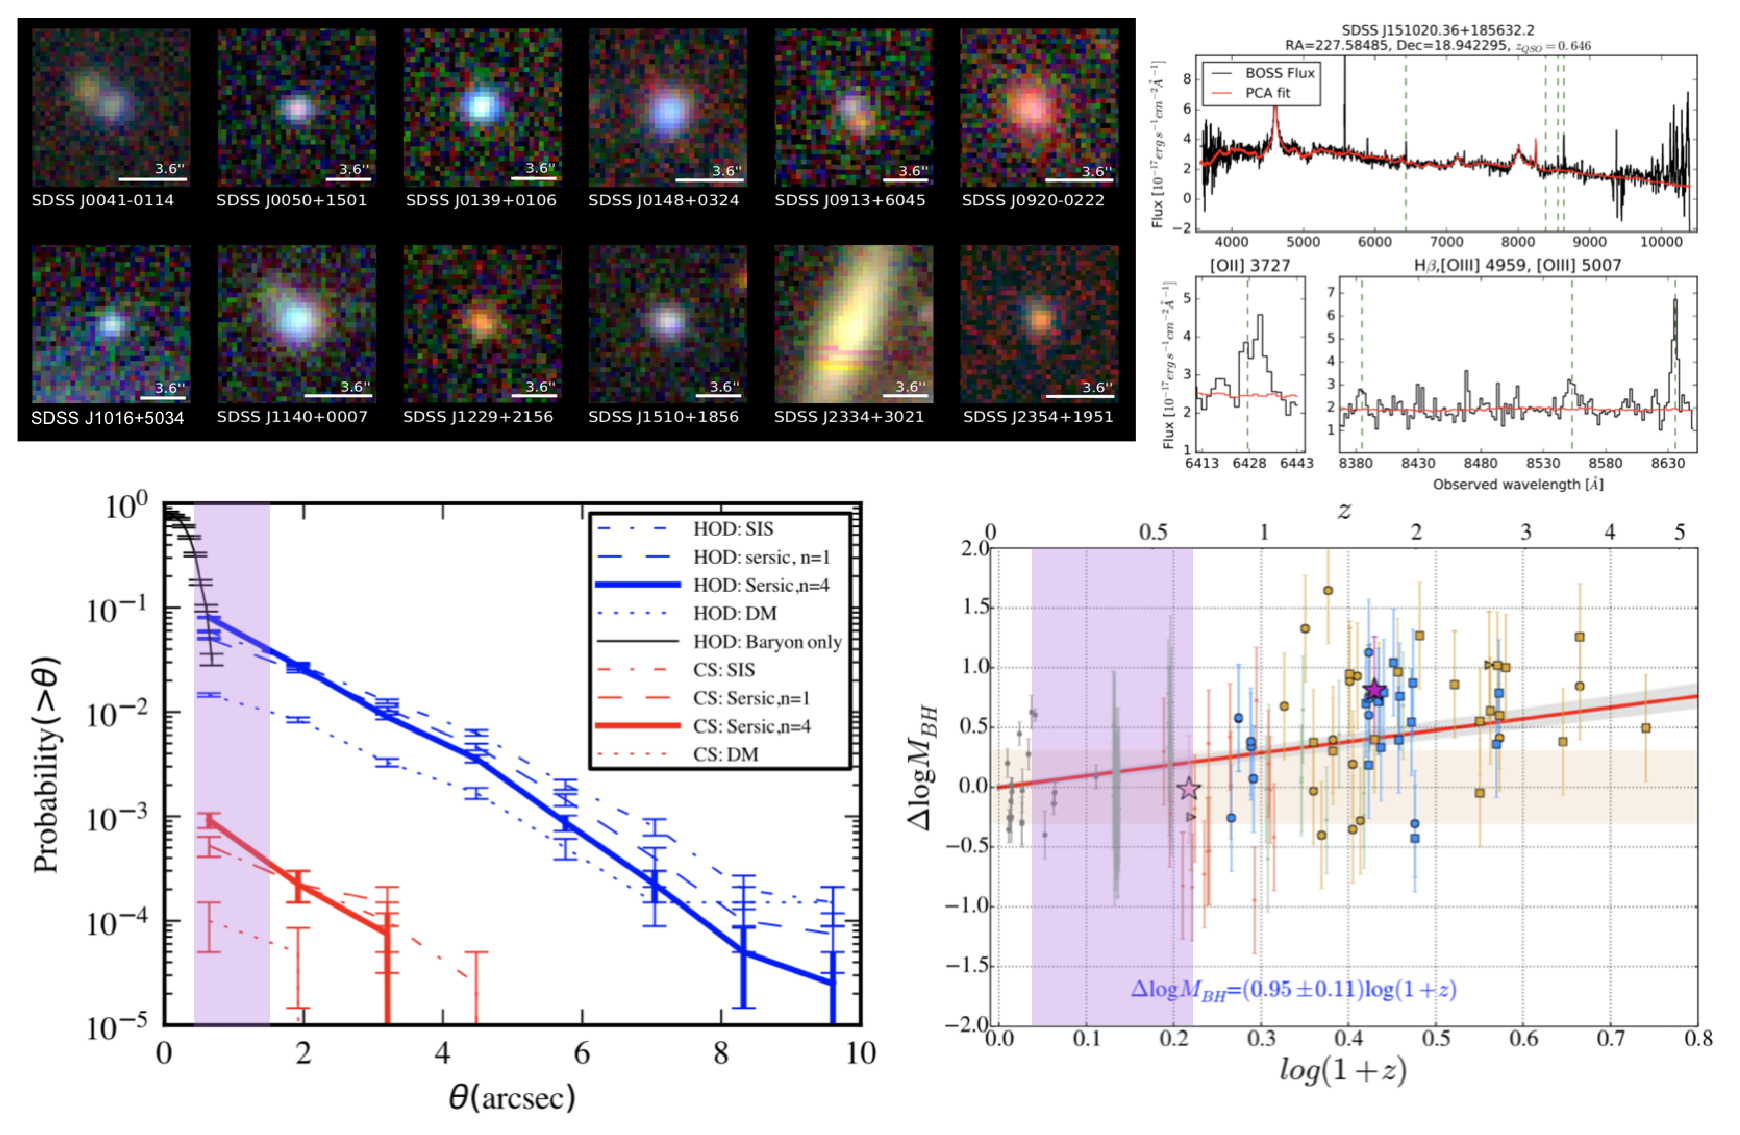
\includegraphics[width=0.95\hsize]{collage.eps}
\end{minipage}
Fig. 1: {\it Top left:} The 9+3 SDSS candidate quasars lensing emission line galaxies and Ly$\alpha$ emitters, from Meyer et al. 2017. {\it Top right:} Example of the spectrum of a foreground quasar showing higher redshift emission lines, from Meyer et al. 2017. {\it Bottom left:} Probability of foreground quasars lensing galaxies, for 2 types of host dark matter halos, from Cen \& Safarzadeh 2017. {\it Bottom right:} Evolution of the offset of $M_{BH}$ in relation to the present day $M_{BH} - L_{\star}$ relation, from the newest compilation in Ding et al. 2017. 
  
{\bf References.} Bolton A.~S., et al., 2008, ApJ, 682, 964-984 $\diamond$ Bonvin V., et al., 2017, MNRAS, 465, 4914 $\diamond$ Courbin, F., et al., A\&A, 516, L12, 2012 $\diamond$ Courbin, F., et al., A\&A, 540, A36, 2012 $\diamond$ Ding X., et al., 2017, MNRAS, 472, 90 $\diamond$ Cen R., et al., 2017, MNRAS, 467, L26 $\diamond$ Gultekin, K. et al., 2009, ApJ, 698, 198 $\diamond$ Guyon et al., 2006, ApJS, 166, 89 $\diamond$ Koopmans et al., 2009, ApJ, 703, L51$\diamond$ Lucey J.~R., et al., MNRAS, 2018 $\diamond$ Meyer R.~A., et al., 2017, arXiv:1711.01184 $\diamond$ More A., et al., 2016, MNRAS, 456, 1595 $\diamond$ Sonnenfeld A., et al., 2018, PASJ, 70, S29 $\diamond$ Oguri M., et al., MNRAS, 439, 2494 $\diamond$ Peng, C., et al., 2007, ApJ, 671, 1098 $\diamond$ Peterson B.~M., 2014, SSRv, 183, 253 $\diamond$ Rusu C.~E., et al., 2016, MNRAS, 458, 2 $\diamond$ Shen et al., 2013, ApJ, 778, 98 $\diamond$ Wong K.~C., et al., 2017, MNRAS, 465, 4895.

\end{document}
